\documentclass{article} % For LaTeX2e
\usepackage{nips13submit_e,times}
\usepackage{hyperref}
\usepackage{url}
\usepackage[ruled,vlined]{algorithm2e}
\usepackage{amsmath}
\usepackage{mathtools} 
\usepackage{float}
\DeclareUnicodeCharacter{FB01}{fi}
%\documentstyle[nips13submit_09,times,art10]{article} % For LaTeX 2.09


\title{Eigenvectors of Metabolic Networks and Gene Expression Profiles: Smoothness and Correlation}


\author{
Yuhou Zhou\\
Department of Computer Science \& Electrical Engineering\\
Jacobs University University\\
28201, Bremen \\
\texttt{yu.zhou@jacobs-university.de} \\
}

% The \author macro works with any number of authors. There are two commands
% used to separate the names and addresses of multiple authors: \And and \AND.
%
% Using \And between authors leaves it to \LaTeX{} to determine where to break
% the lines. Using \AND forces a line break at that point. So, if \LaTeX{}
% puts 3 of 4 authors names on the first line, and the last on the second
% line, try using \AND instead of \And before the third author name.

\newcommand{\fix}{\marginpar{FIX}}
\newcommand{\new}{\marginpar{NEW}}

\nipsfinalcopy % Uncomment for camera-ready version

\begin{document}


\maketitle

\begin{abstract}
 I implement a workflow \footnote{Available on \textit{https://github.com/yuhouzhou/eigengene}} to quantitatively assess smoothness of a colored graph and check the correlation between eigenvectors of a metabolic network and gene expression profiles. Rapaport et al. use gene network information as a priori to gene expression profoile analysis. This project expand previous work by quantifying the smoothness of a colored graph and checking correlation between eigenvectors of the metabolic network and gene expression profiles. The workflow of the experiment includes data preprocessing, plotting metabolic network, quantifying smoothness, compute correlation coefficients. Finally, a conclusion about these two points are drawn and some future work is discussed. 
\end{abstract}

\section{Introduction}
Analysing gene expression profiles is a way to understand genetic phenomena. However, connecting genes and biological significance is a difficult task. By including a priori knowledge from a gene network to gene expression profiles can facilitate the process of understanding biological significance of genes, dissecting the genes responsible for a phenotype \cite{rapaport_classification_2007}. By looking at eigenvalues and eigenvectors of the Laplacian matrix of a gene network, we can attenuate high-frequency component of the gene network, and a distance metric can be defined based on it. In this report, Section ~\ref{section:background-start} to section ~\ref{section:background-end} give some background knowledge about spectral graphy theory, network biology, and BiGG database and GEO Omnibus database. Section ~\ref{section:experiments} shows the pipeline of the experiments and their results. Section ~\ref{section:conclusions} restate the conclusions from the experiments, and section ~\ref{section:discussion} opens the discussion for the work which could be further done.

\section{Related Work}
Gene network is any graph with genes as vertices, and edges between genes can represent various biological information. Metabolic gene networks use genes, which encode enzymes, as nodes, and the edges between two genes indicate that the product of a reaction catalysed by the enzyme of the first gene is the substrate of the reaction catalysed by the enzyme of the second gene. Beside the metabolic gene networks, there are gene regulatory network, protein-protein interaction network, gene co-expression networks, signaling networks, etc.

Spectral graph theory starts by associating matrices to graphs — notably, the adjacency matrix and the Laplacian matrix. The general theme is then, firstly, to compute or estimate the eigenvalues of such matrices, and secondly, to relate the eigenvalues to structural properties of graphs \cite{nica_brief_2018}.

Rapaport et al. proposed a method to integrate a priori, the knowledge of a gene network, in the analysis of gene expression data \cite{rapaport_classification_2007}. In the paper, the eigenvalues and eigenvectors of Laplacian from a metabolic network are firstly derived as the priori. They defined a metric which measures the distance between gene expression profiles. This metric uses the eigenvalues to attenuate high frequency components of the metabolic network. The paper further illustrates how such distance metric can be used for classification or regression purpose. 

\section{Spectral Decomposition} \label{section:background-start}
Spectral graph theory has a long history. Both algebraic method and geometric method utilize eigenvalues of  the graph matrices. One of the main goals in graph theory is to deduce the principal properties and structure of a graph from its graph spectrum. The Laplacian of the graph $G$ is the $n * n$ matrix, let $d_v$ denote the degree of the vertex $v$ \cite{chung_spectral_1997}:

\[
    L (u, v) = 
    \begin{cases}
        d_v & if\ u = v,\\
        -1 & if\ u\ and\ v\ are\ adjacent,\\
        0 & otherwise.
    \end{cases}
    \]\\

$L$ is the key concept of the spectral graph theory, It has some important properties: It is symmetric, positive semidefinite, and singular; Its eigenvalues $\lambda_{i}$ are larger than $0$, and the  the smallest eigenvalue $\lambda_0 = 0$. 

\section{Network Biology}
There are many different forms of interaction happening in biological organisms. These different kinds of interactions can be described as networks. It provides a mathematical representation of such connections. Adjacency matrix and Laplacian matrix are commonly used to study propoerties of networks. In order to understand networks better, some basic attributes of it should be known \cite{barabasi_network_2004}.

\textbf{Veterx and Edge:} 
A network is an abstract representation of a number of points connected by lines. Each point is usually called a vertex, and the lines are edges. In a terrestrial transportation network, some geographical locations can be vertices and the roads between them are edges. In protein-protein interaction networks, vertices are proteins and links represents mutual interactive relationship.

\textbf{Directed or Undirected:}
Depending on the nature of the interactions, networks can be directed or undirected. In the above examples. A terrestrial transportation network can have roads which allow only one direction driving, so in many cases it is beneficiary to consider direction of edges in analysis. In a protein interaction network, the edges represent mutual relationship among proteins. Thus, such network is undirected.

\textbf{Degree:}
The most elementary characteristic of a node is its degree, which tells us how many edges the vertex has to other vertices. In directed graph, for each node, the degree of one vertex is divided into incoming degree and outgoing degree. For the mentioned transportation network, for certain location, the roads which allow transportation coming in make incoming edges, and the number of them is the incoming degree.

\subsection{Gene Network}
In this project, experiments about the Laplacian property of a specific kind of biological network, gene network, was studied. Gene network is any graph with genes as vertices, and edges between genes can represent various biological information. Gene regulatory networks (DNA-protein interaction network) describes transcription factors, proteins binding to DNA, regulate the activities of genes. Metabolic gene networks use genes, which encode enzymes, as nodes, and the edges between two genes indicate that the product of a reaction catalysed by the enzyme of the first gene is the substrate of the reaction catalysed by the enzyme of the second gene. The main gene network used in this project is the metabolic network of yeast.

\section{Data Source} \label{section:background-end}
BiGG database contains a repository of high-quality, manually-curated genome-scale metabolic models (GEM), which can be used to predict metabolic pathway usage and growth phenotypes. BiGG centralized more than 75 GEM's \cite{king_bigg_2016}. The data set of a organism can be downloaded on its website in \textit{xml, json,} and \textit{mat} formats. A python library (BiGG\footnote{Available on \textit{https://github.com/SBRG/bigg\_models}}) is also provided for accessing the database programmatically. The syntax of the data set is intuitive and it can be extracted to structured form with little effort. Comparing to more extensive knowledge base, such as Kyoto Encyclopedia of Genes and Genomes (KEGG), the process of constructing metabolic network is more straightforward. 

The Gene Expression Omnibus (GEO) database stores high-throughput gene expression profile data sets with detailed descriptions. \cite{clough_gene_2016} To recognize different records, a naming convention is applied. Series (GSExxx), Sample (GSMxxx), Platform (GPLxxx) and data set (GDSxxx). "A Platform record is composed of a summary description of the array or sequence and, for array-based Platforms, a data table defining the array template. A Sample record describes the conditions under which an individual Sample was handled, the manipulations it underwent, and the measurements derived from it. A Series record links together a group of related Samples and provides a focal point and description of the whole study. A fourth record type, referred to as data sets (GDSxxx), are assembled by the GEO curation staff from the three primary records."

\section{Experiments} \label{section:experiments}
The data sets are downloaded from BiGG models. The main model is iND750 for Saccharomyces cerevisiae S288C, other models, used to compare with the main one, are iAM\_pb448 for plasmodium berghei, iEC1344\_C for Escherichia coli C, iMM904 for Saccharomyces cerevisiae S288C. Models are stored in JSON format.

\subsection{Data Preprocessing for Metabolic Network}
Every model contains 6 keys, namely "metabolites", "reactions", "genes", "id", "compartments", and "version". Every BiGG model has an ID, and that contains three parts: the two capital letters stands for the first letter of author's last names. the number attached indicated the number of genes in the model. 

The "compartments" entry shows the abbreviation of the naming convention for "reactions" and "metabolites". For instance, 'c' stands for 'cytosol', 'g' stands for 'golgi apparatus', and 'e' stands for 'extracellular space'. Knowing this, the comparment where  some rection takes place can be informed, such as "EX\_met\_\_L\_e" is located at extracellular space.

The "metabolites" entry contains a list of metabolites involved in all the reactions. Important keys for preprocessing "id", "compartment" and "formula". The "compartment" entry can be used to study the network in a specific compartment, and by defining some rules, the "formula" helps filter out inorganic substances and leave the enzymes.

The "reaction" entry contains a list of information of reactions. Every reaction are represented as a dictionary. One of the important keys for preprocesing is "metabolites" (not the "metabolites" entry) which comprise the metabolites ID and their stoichiometry of the reaction. metabolite ID can be searched in "metabolites" entry. The positive sign of the stoichiometry means the metabolite is the product of the reaction, the negative sign means the substrate. The value of "gene\_reaction\_rule" are the ID's of genes which rule the reaction.

The "gene" entry contains a list of genes of the model. The important keys for preprocessing is "id".

\begin{algorithm}[H]
\SetAlgoLined
\KwResult{edges}
 initialize an empty table $T$\;
 \For {gene in "genes" entry}{
    add gene name as index the table $T$\;
    \For {reaction in "reactions" entry}{
    \eIf{the reaction is ruled by the gene}
    {record the reaction and its substrates and products to the gene\;
    exclude inorganic substance\;}{pass}
    }
 }
 
 \For{gene $a$ in $T$}{
  \For{gene $b$ in $T$}{
  \eIf{substrate of $a$ is product of $b$}{gene $a$ and gene $b$ have an edge between them}{pass}
  }
 }
 
 \caption{Extract edges between genes}
\end{algorithm}

\subsection{Plot Metabolic Network}
After the prepocessing, there are 6001 edges among 684 nodes. The experiment use Python library NetworkX and Matplotlib to draw the graph. The Laplacian matrix can be easily extracted by the NetwrokX method \textit{laplacian\_matrix()}.

The $684*684$ Laplacian matrix of the iND750 network is
\begin{equation*}
\begin{aligned}
\begin{bmatrix}
12 & 0 & 0 & \dots & 0 & 0 & -1\\
0 & 30 & 0 & \dots & 0 & 0 & 0 \\
0 & 0 & 30 & \dots & 0 & 0 & 0 \\
\vdots & \vdots & \vdots & \vdots & \vdots & \vdots &\vdots\\
0 & 0 & 0 & \dots & 3 & 0 & 0 \\
0 & 0 & 0 & \dots & 0 & 12& 0 \\
-1 & 0 & 0 & \dots & 0 & 0 & 26
\end{bmatrix}
\end{aligned}
\end{equation*}
The eigenvalues and eigenvectors can be computed by \textit{numpy.linalg.eig()}. We, following Rapaport's notation, denote eigenvalues by $0 = \lambda_0 \leq \dots \lambda_k \dots \leq \lambda_{n-1}$ and the corresponding eigenvectors by $e_1,\dots,e_n$, where $n$ is the number of nodes in the network. The entries of an eigenvector are used to color the network. The color map is defined as: positive coefficients are marked in red, negative coefficients are in blue, and the intensity of the colour reflects the absolute values of the coefficients. The plot showing an example of Laplacian eigenvectors is presented on Figure ~\ref{fig:iND750-4}. The workflow is repeated for iAM\_Pb448, iEC1344, Recon3D models, showing on ~\ref{fig:iAM_Pb448-4}, ~\ref{fig:iEC1344_C-4}, ~\ref{fig:Recon3D-4}. They show a similar pattern of smoothness decreasing; only Recon3D model is rather homogeneous even with the largest eigenvalue. This was further explain in Section ~\ref{section:quantify-smoothness} A plot with a fixed step between eigenvalues to show the decreasing of smoothness is on Figure ~\ref{fig:iND750}. 
\begin{figure}[H]
      \graphicspath{ {images/} }
      \begin{center}
            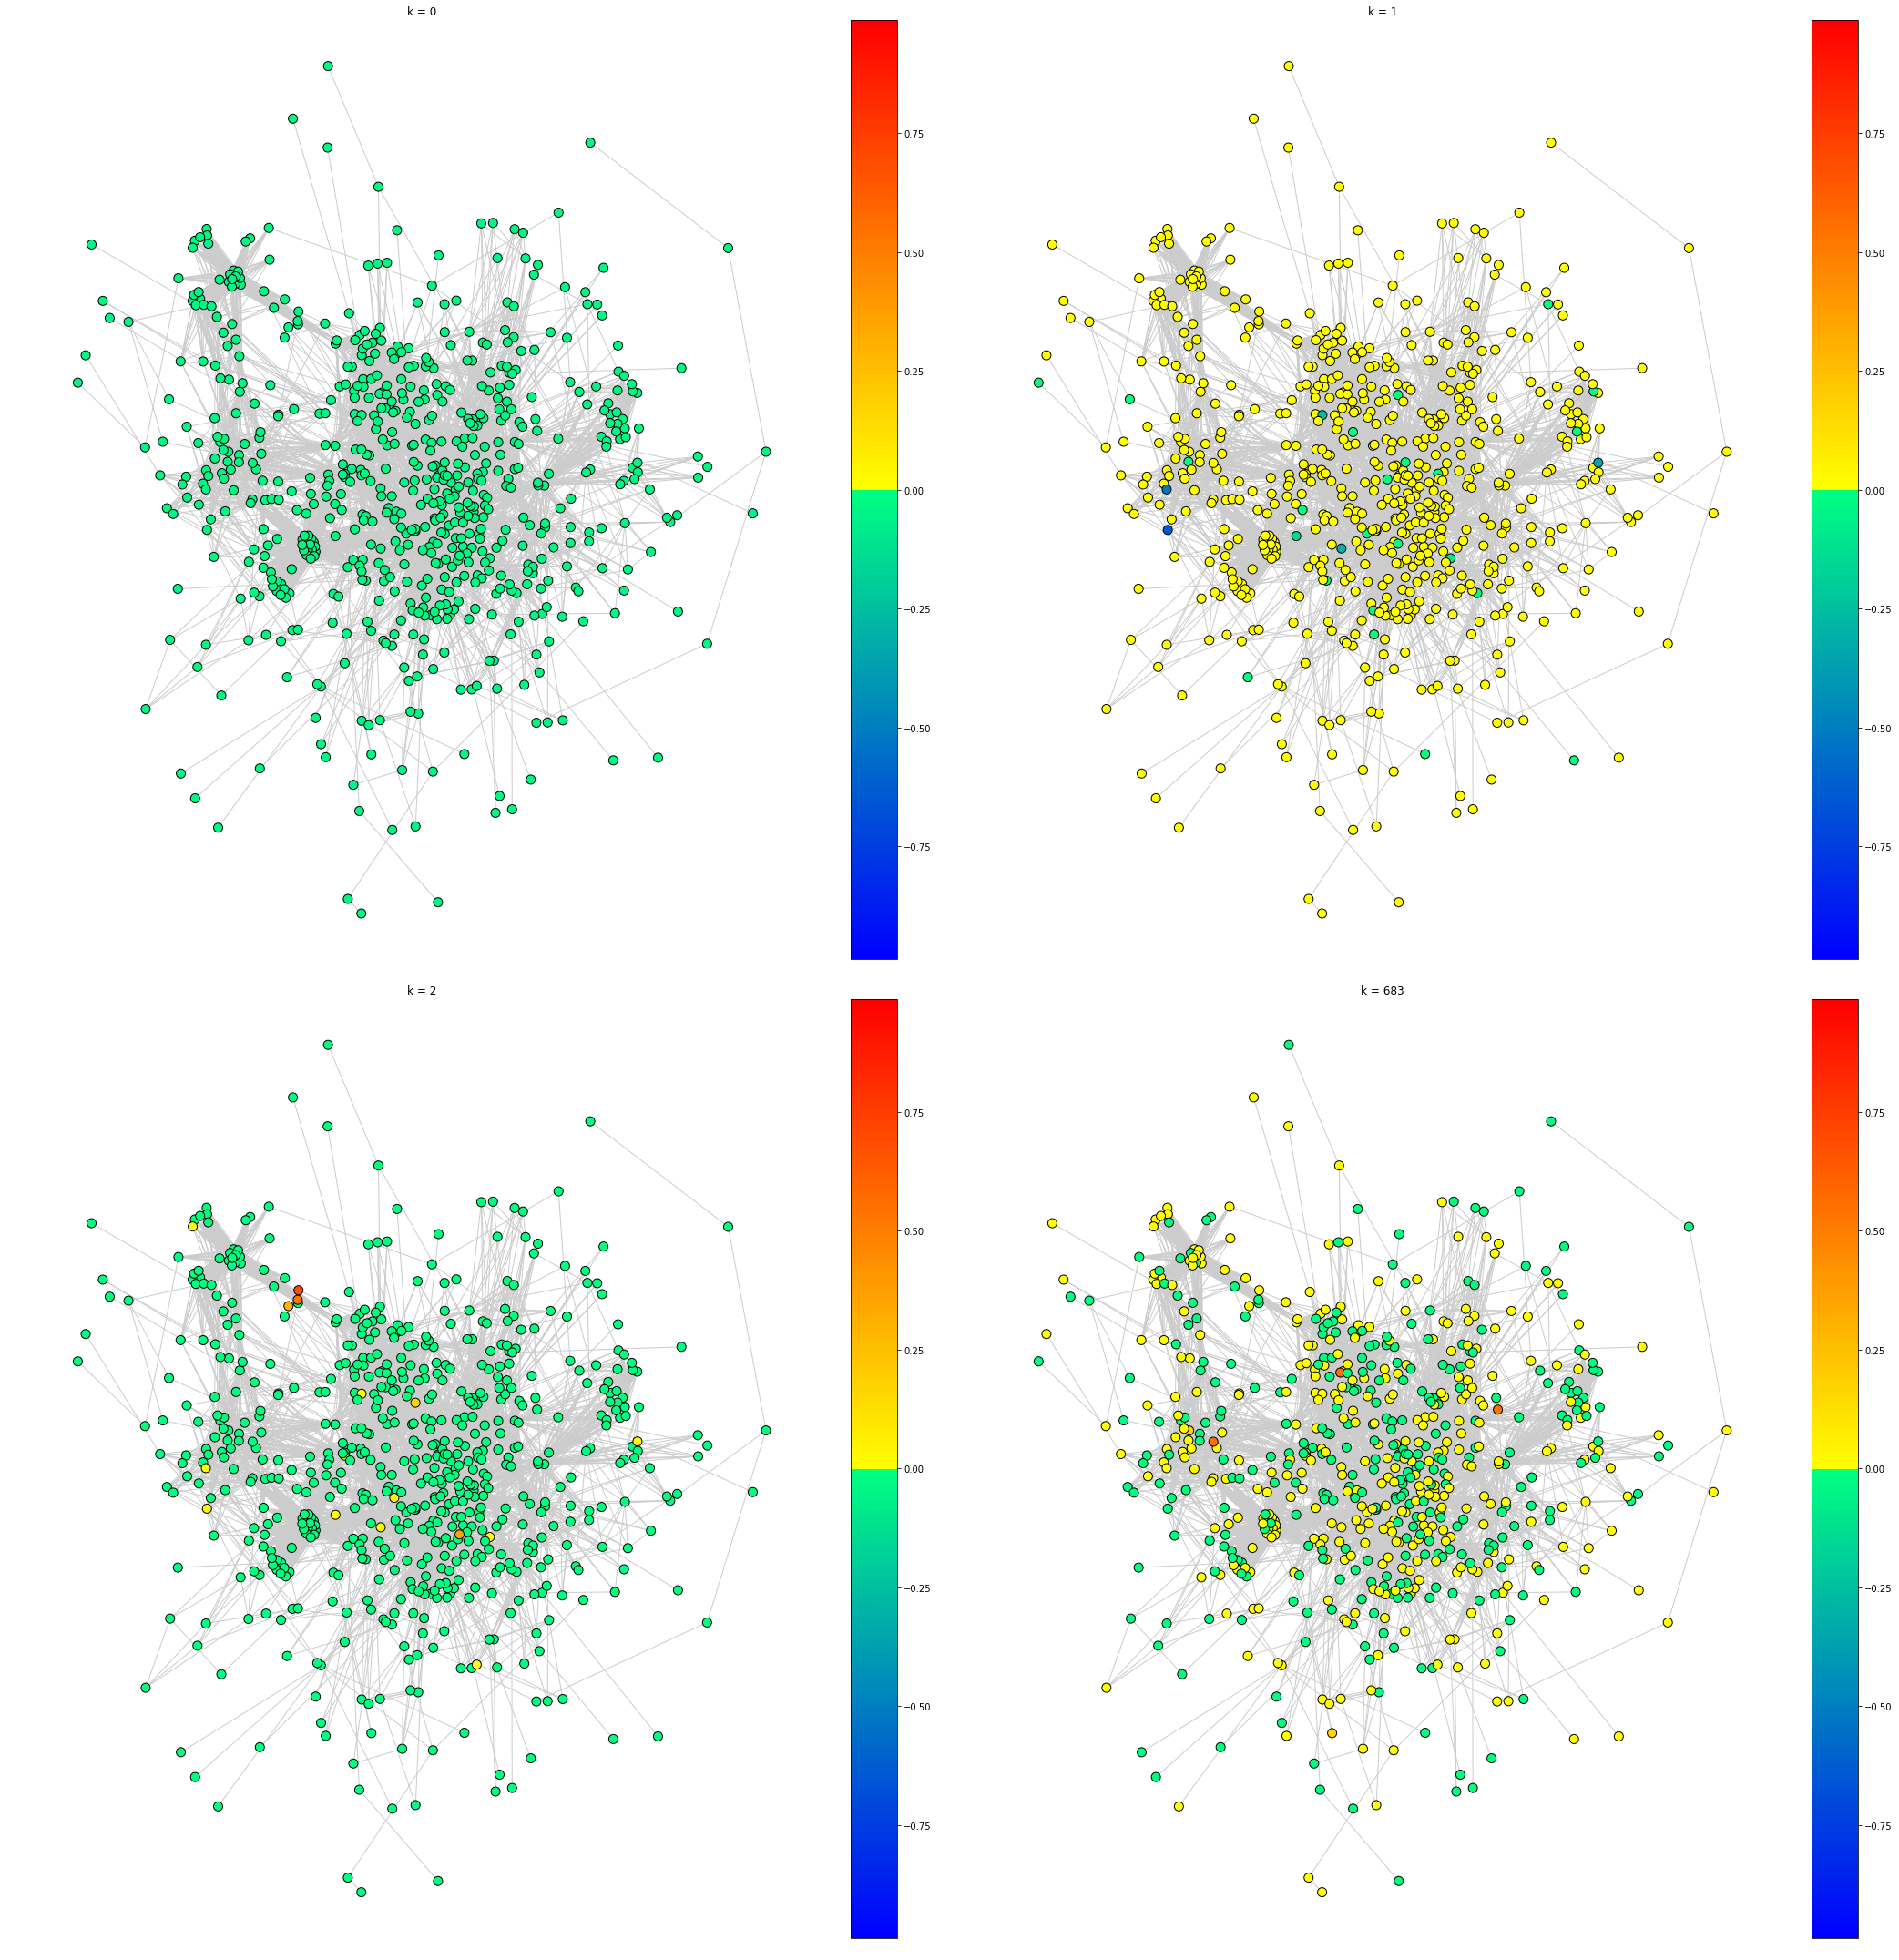
\includegraphics[scale=0.2]{iND750-4.png}
      \end{center}
      \caption{\textbf{Example of Laplacian eigenvectors.} On the upper-left side is the eigenvector associated with the smallest eigenvalue, on the upper-right side the one associated with the second smallest eigenvalues, on the lower-left side, the one associated with the third smallest eigenvalue while on the lower-right side is the one associated with the largest eigenvalue. The larger the eigenvalue, the less smooth the corresponding eigenvector.}
      \label{fig:iND750-4}
\end{figure}

\subsection{Quantify Smoothness} \label{section:quantify-smoothness}
Since the decreasing of smoothness is hard to distinguish between subplots by eyes when $k$ is large, a quantitative way to assess the smoothness of the graph needs to be proposed. After remove the color bar and titles of the subplots, we use the file size of saved subplots to represent the homogeneity of the graph. The relation between indices $k$ and the file sizes $s$ are plotted as Figure ~\ref{fig:iND750-smoothness}. The x axis is standardized by $ k = k / n$, and the file size is standardized by $s = \frac{s - min(S)}{max(S)}$, where $S$ is the set of file sizes. After standardisation, x and y axes have the range from $0$ to $1$.

\begin{figure}[!htb]
\minipage{0.32\textwidth}
  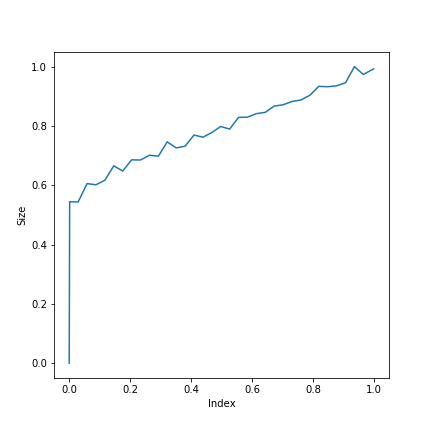
\includegraphics[width=\linewidth]{images/iND750-smoothness.png}
  \caption{iND750 model (Saccharomyces cerevisiae S288C) smoothness change}\label{fig:iND750-smoothness}
\endminipage\hfill
\minipage{0.32\textwidth}
  \includegraphics[width=\linewidth]{images/iAM_Pb448-smoothness.png}
  \caption{iAM\_Pb448 model (Plasmodium berghei) smoothness change}\label{fig:iAM_Pb448-smoothness}
\endminipage\hfill
\minipage{0.32\textwidth}%
  \includegraphics[width=\linewidth]{images/Recon3D-smoothness.png}
  \caption{Recon3D model (Homo sapiens) smoothness change}\label{fig:Recon3D-smoothness}
\endminipage
\end{figure}

In order to check if the pattern of smoothness decreasing exists also in other metabolic network from different organisms. Above workflow was repeated for iAM\_Pb448 and Recon3D models. Their results are showed on Figure ~\ref{fig:iAM_Pb448-smoothness} and Figure ~\ref{fig:Recon3D-smoothness}. Among different species, they are showing a similar pattern that the rate of decrease is large before first 10\% of the indices, and then the rate become smaller. The previously observed homogeneous of Recon3D model with the largest eigenvalue is explained by the sudden drop of the y value on the end of x axis.

\subsection{Gene Expression Profile}
Gene expression profiles are downloaded from GEO database. In this experiment, one microarray data set "Expression data of Saccharomyces cerevisiae treated with clioquinol" \cite{noauthor_geo_nodate} and one high-throughput sequencing data set "Gene expression analysis using RNA Sequencing of the Saccharomyces cerevisiae BY4741 H4-T30 and S47 mutant strains upon heat and osmotic stress" \cite{noauthor_geo_nodate-1} are used. The data cleaning was performed to find the common gene in both metabolic network and gene expression profile. The visualization of the gene expression profiles are on Figure ~\ref{fig:iND750-expression} and Figure ~\ref{fig:iND750-rna-seq}.

\begin{figure}[H]
      \graphicspath{ {images/} }
      \begin{center}
            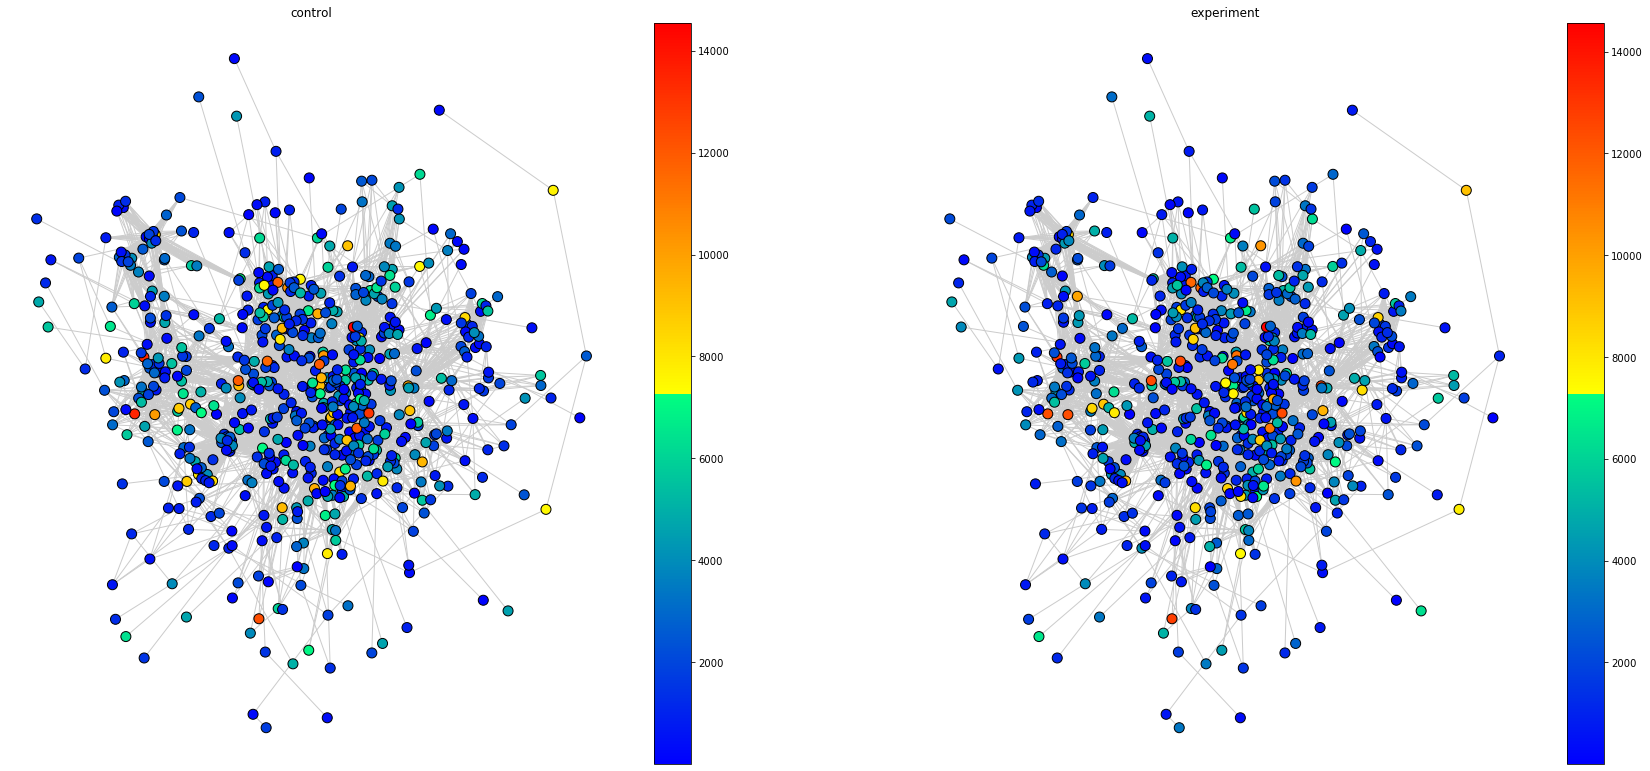
\includegraphics[scale=0.2]{images/iND750-expression.png}
      \end{center}
      \caption{\textbf{iND750 microarray data set.} Expression data of Saccharomyces cerevisiae treated with clioquinol.}
      \label{fig:iND750-expression}
\end{figure}

\begin{figure}[H]
      \graphicspath{ {images/} }
      \begin{center}
            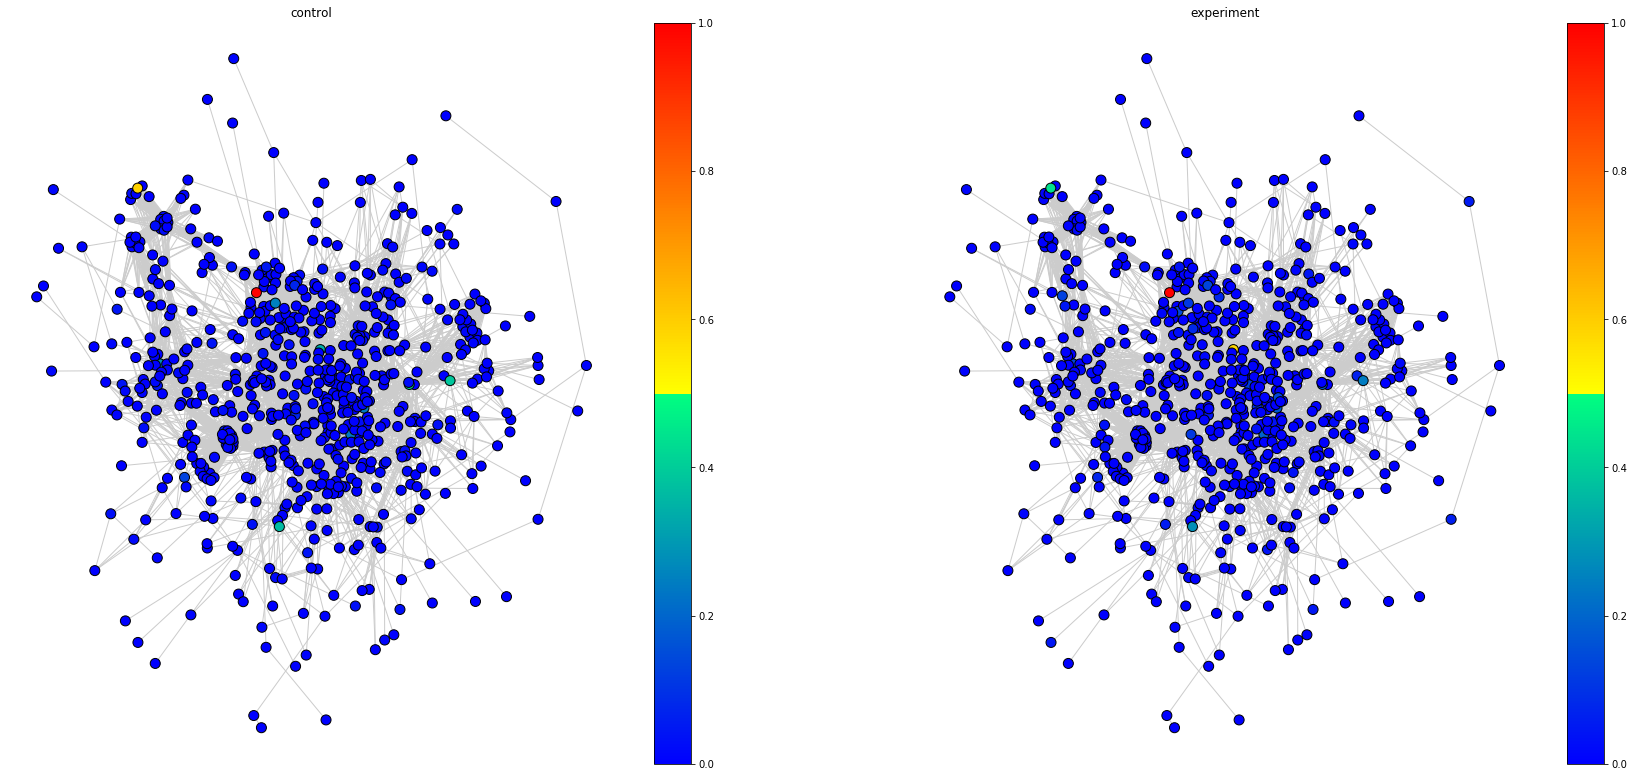
\includegraphics[scale=0.2]{images/iND750-rna-exp.png}
      \end{center}
      \caption{\textbf{iND750 high-throughput sequencing data set.} Gene expression analysis using RNA Sequencing of the Saccharomyces cerevisiae BY4741 H4-T30 and S47 mutant strains upon heat and osmotic stress}
      \label{fig:iND750-rna-seq}
\end{figure}

\subsection{Correlation between Eigenvectors and Gene Expression Profiles}
The correlation between eigenvectors and gene expression profiles are based on Pearson correlation coefficient and Spearman's correlation coefficient. Pearson correlation coefficient is defined as $r=\frac{cov_{xy}}{s_xs_y}=\frac{\sum(x_i-\overline{x})((y_i-\overline{y})}{(N-1)s_xs_y}$, where $N$ is the number of samples, $s$ is the standard deviation. It is the standardized covariance whose range is between $-1$ and $1$. Spearman's correlation coefficient first takes the rank of the variables and applies the rank to Pearson function. 

The final coefficient is the maximum values of all coefficients (both Pearson and Spearman's) between each eigenvector and the gene expression profile vector. The result is shown on the Table ~\ref{table:coeff}.

\begin{table}[h!]
\centering
\begin{tabular}{ |p{4cm}||p{4cm}|p{4cm}| }
%  \hline
%  \multicolumn{3}{|c|}{Maximum Correlation Coefficient} \\
 \hline
 data set & Correlation coefficient & P value \\
 \hline
 Miscroarray   & 0.1897602896124568 & 2.7242330200126107e-05\\
 RNA sequencing & 0.2717323999012909 & 6.592013500421056e-13\\
 \hline
\end{tabular}
\caption{Maximum Correlation Coefficient}
\label{table:coeff}
\end{table}

In order to validate the result, the entries of gene expression profile vector are shuffled, and then the shuffled vector is compared to the eigenvectors. The process is conducted for 100 times, and thus we yield a distribution of the result. It is shown on Figure ~\ref{fig:coe-distr-micros} and Figure ~\ref{fig:coe-distr-rna}.

\begin{figure}[H]
      \graphicspath{ {images/} }
      \begin{center}
            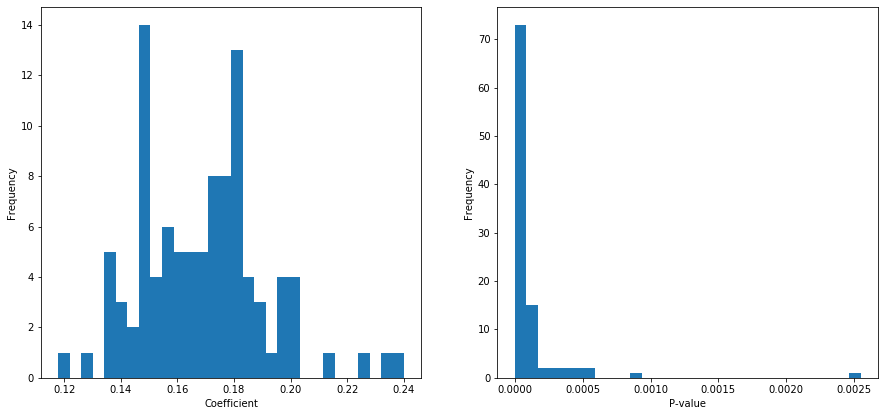
\includegraphics[scale=0.4]{images/coe-distr-microa.png}
      \end{center}
      \caption{\textbf{Distibution of coefficients and p-values of iND750 microarray data set}}
      \label{fig:coe-distr-micros}
\end{figure}

\begin{figure}[H]
      \graphicspath{ {images/} }
      \begin{center}
            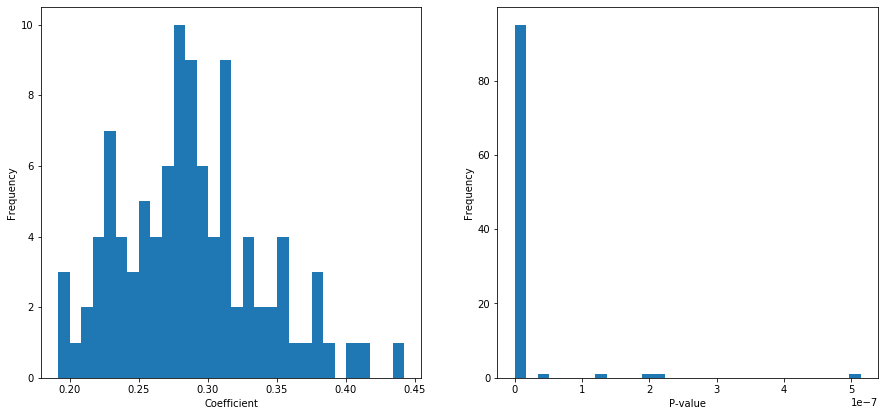
\includegraphics[scale=0.4]{images/coe-distr-rna.png}
      \end{center}
      \caption{\textbf{Distibution of coefficients and p-values of iND750 data set high-throughput sequencing data set.} }
      \label{fig:coe-distr-rna}
\end{figure}

The two modes of the distribution of microarray coefficient are $0.15$ and $0.18$, the mode of the distribution of RNA-sequencing coefficient is around $0.275$. The modes are close to the coefficients, which are got from comparing gene expression profiles and eigenvectors, so we cannot object that the correlated coefficient are insignificant, and the maximum value is yield by coincidence. The conclusion is that the eigenvectors are not significantly correlated with gene expression profiles.

\section{Conclusions} \label{section:conclusions}
From the experiment results, I conclude that the smoothness is overall decreasing, when colored graphs use eigenvectors corresponding to larger eigenvalues. The decreasing rate is high before around ten percent. After the plump of the rate, it declines slowly. There is little difference between species, in terms of such smoothness decreasing pattern. 

The correlation between the eigenvectors and gene expression profiles is weak, because the correlation coefficient is falling into the interval around the mode of correlation coefficient distribution of randomly shuffled gene expression vectors.

\section{Discussion} \label{section:discussion}
In this project, only undirected graphs are considered. A Directed graph (digraph) also can be used to describe metabolic network, as in a chemical reaction, substrates and products are normally not reversible. Akman et al. introduced how Spectral Functional-Digraph Theory can be applied to Gene Regulatory Network. \cite{akman_spectral_2018} The method studies adjacency matrix of the directed graph instead of Laplacian matrix properties. A directed graph can be presented not only by wiring diagram but also phase space, which is more tractable. Considering adjacency matrix and phase space for further analysis is promising.

\section*{Acknowledgements}
This work is mentored by Professor Marc-Thorsten Hütt. I thank him for giving me a guiding hand, and his opening to my mistakes and inexperience. I could not implement this project successfully and have the inspiration to explore more in the field, without his patient mentoring and careful explanation.

\section{Supplementary}
% \begin{figure}[!htb]
% \minipage{0.32\textwidth}
%   \includegraphics[width=\linewidth]{images/iAM_Pb448-4.png}
%   \caption{iAM\_Pb448 metabolic network}\label{fig:iAM_Pb448-4}
% \endminipage\hfill
% \minipage{0.32\textwidth}
%   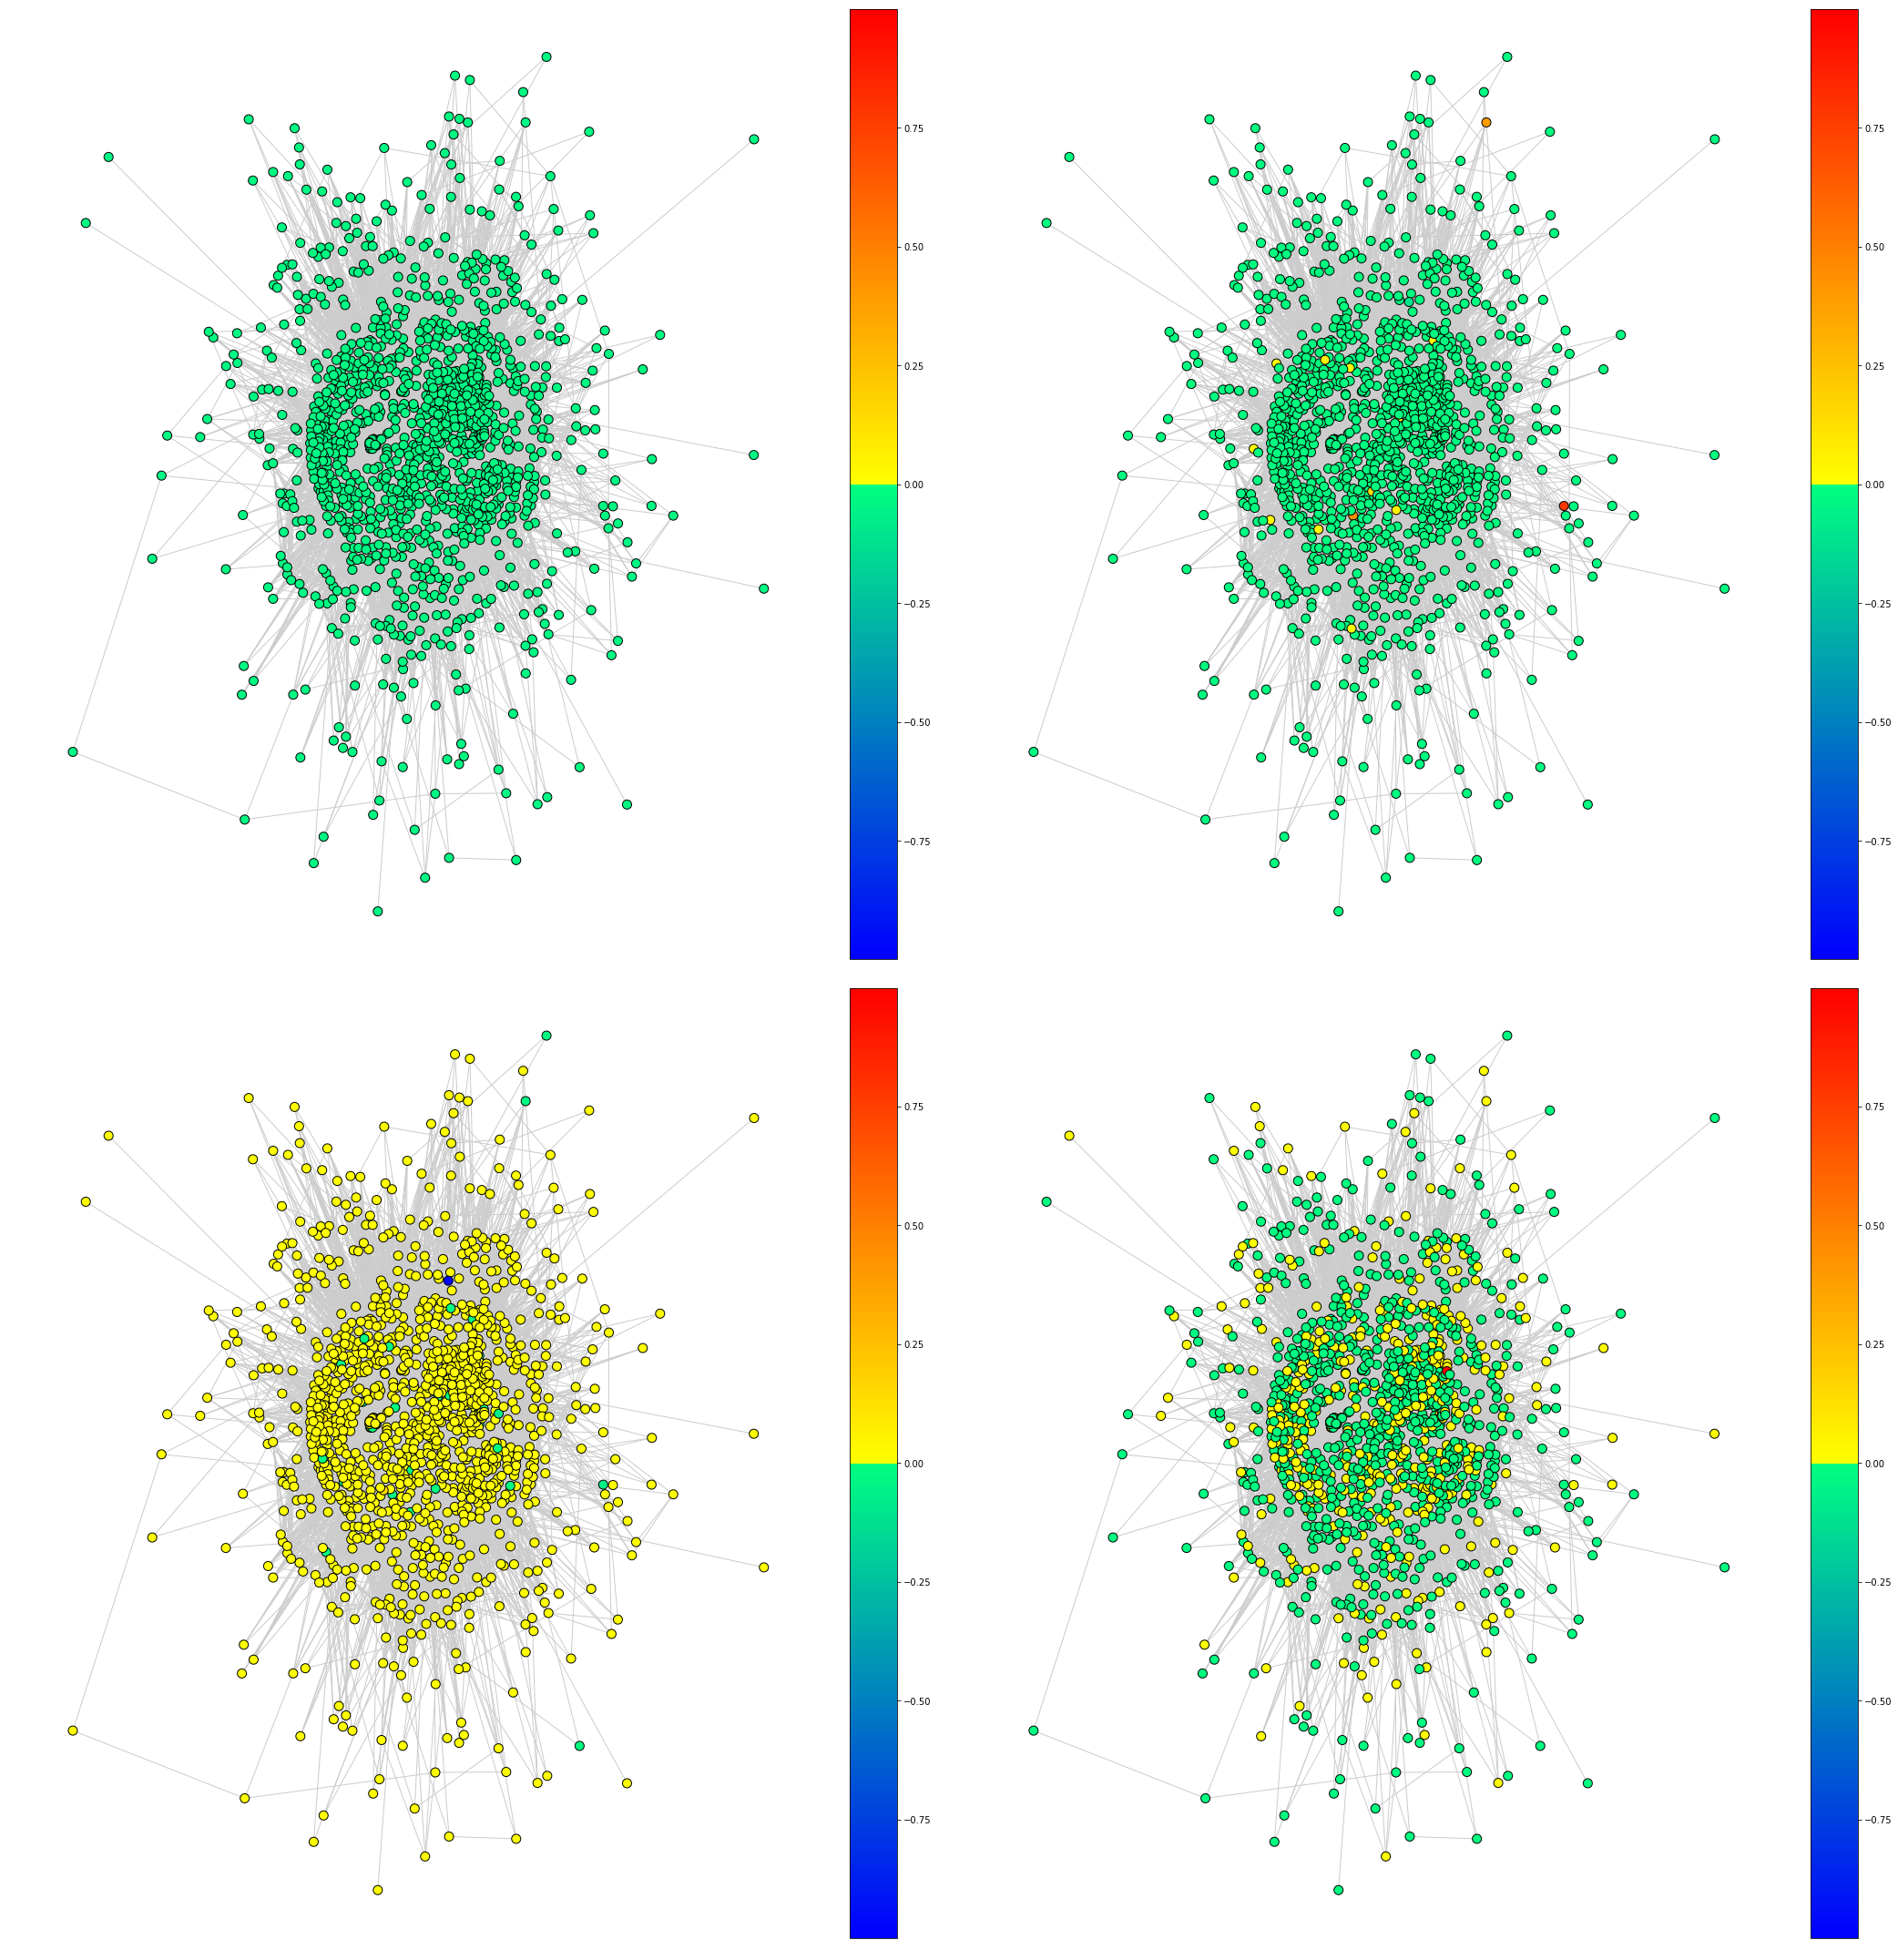
\includegraphics[width=\linewidth]{images/iEC1344_C-4.png}
%   \caption{iEC1344 metabolic network}\label{fig:iEC1344_C-4}
% \endminipage\hfill
% \minipage{0.32\textwidth}%
%   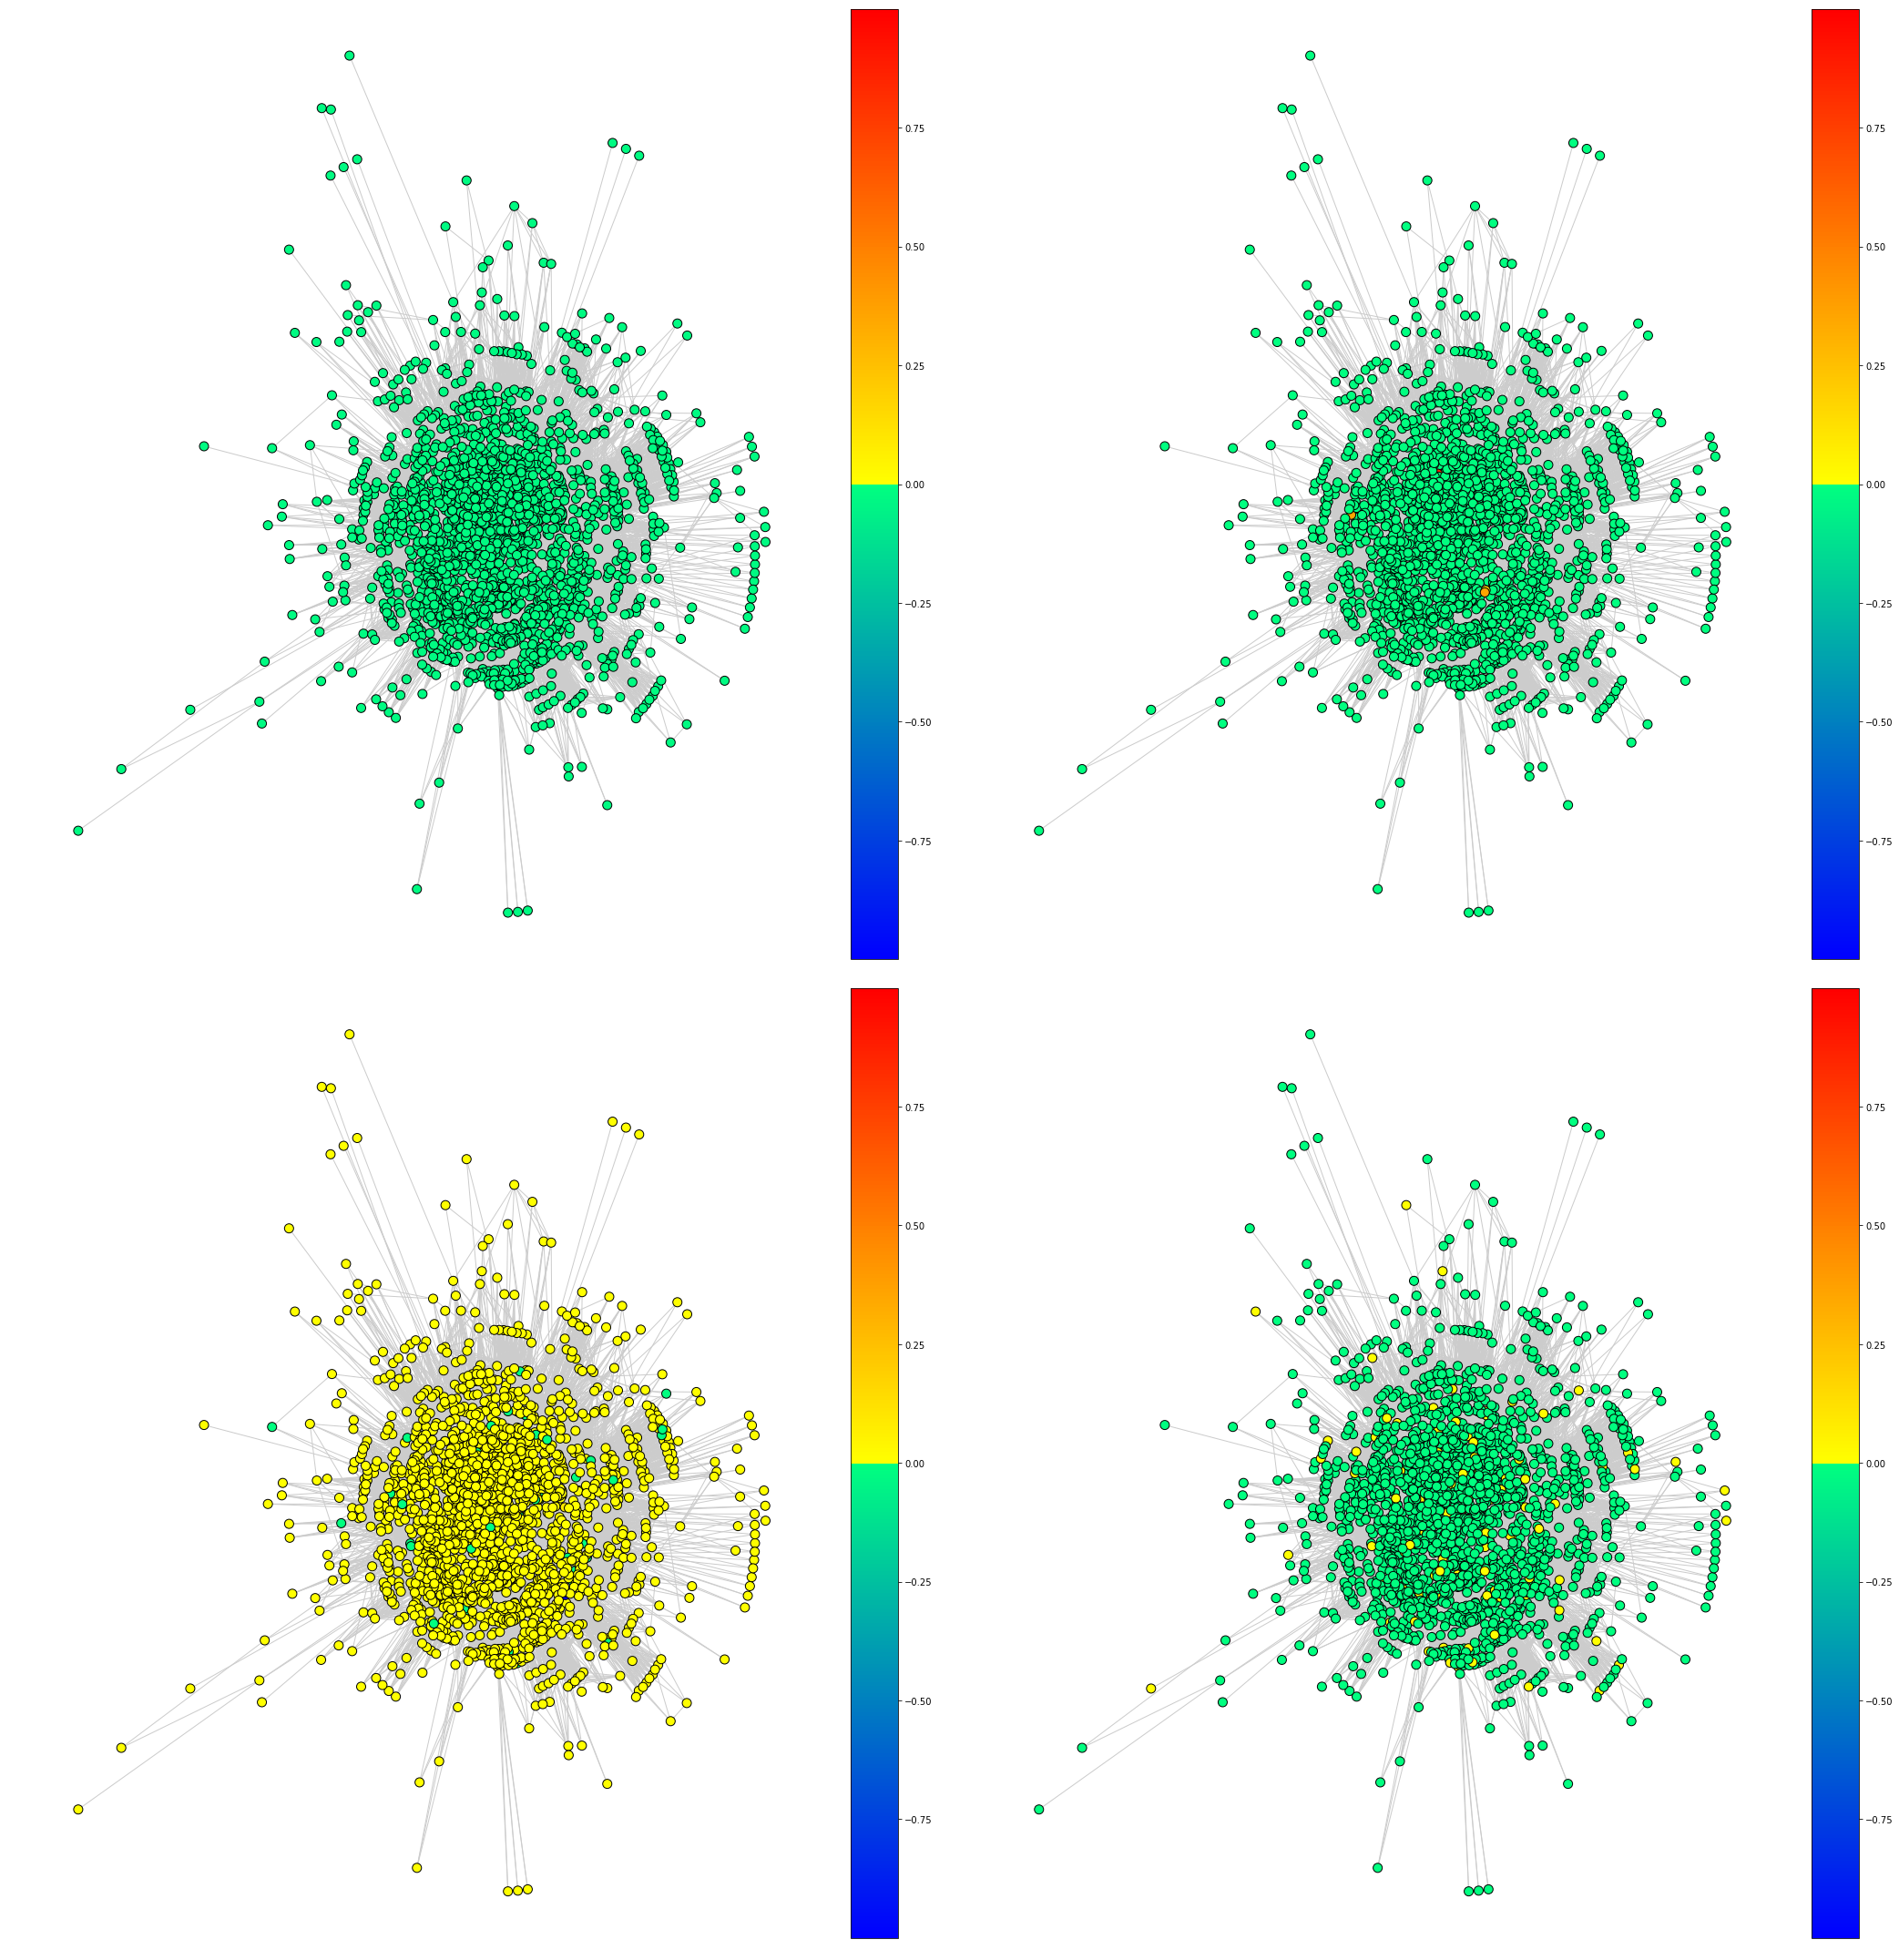
\includegraphics[width=\linewidth]{images/Recon3D-4.png}
%   \caption{Recon3D metabolic network}\label{fig:Recon3D-4}
% \endminipage
% \end{figure}

\begin{figure}[H]
      \graphicspath{ {images/} }
      \begin{center}
            \includegraphics[scale=0.2]{images/iAM_Pb448-4.png}
      \end{center}
      \caption{iAM\_Pb448 metabolic network}\label{fig:iAM_Pb448-4}
\end{figure}

\begin{figure}[H]
      \graphicspath{ {images/} }
      \begin{center}
            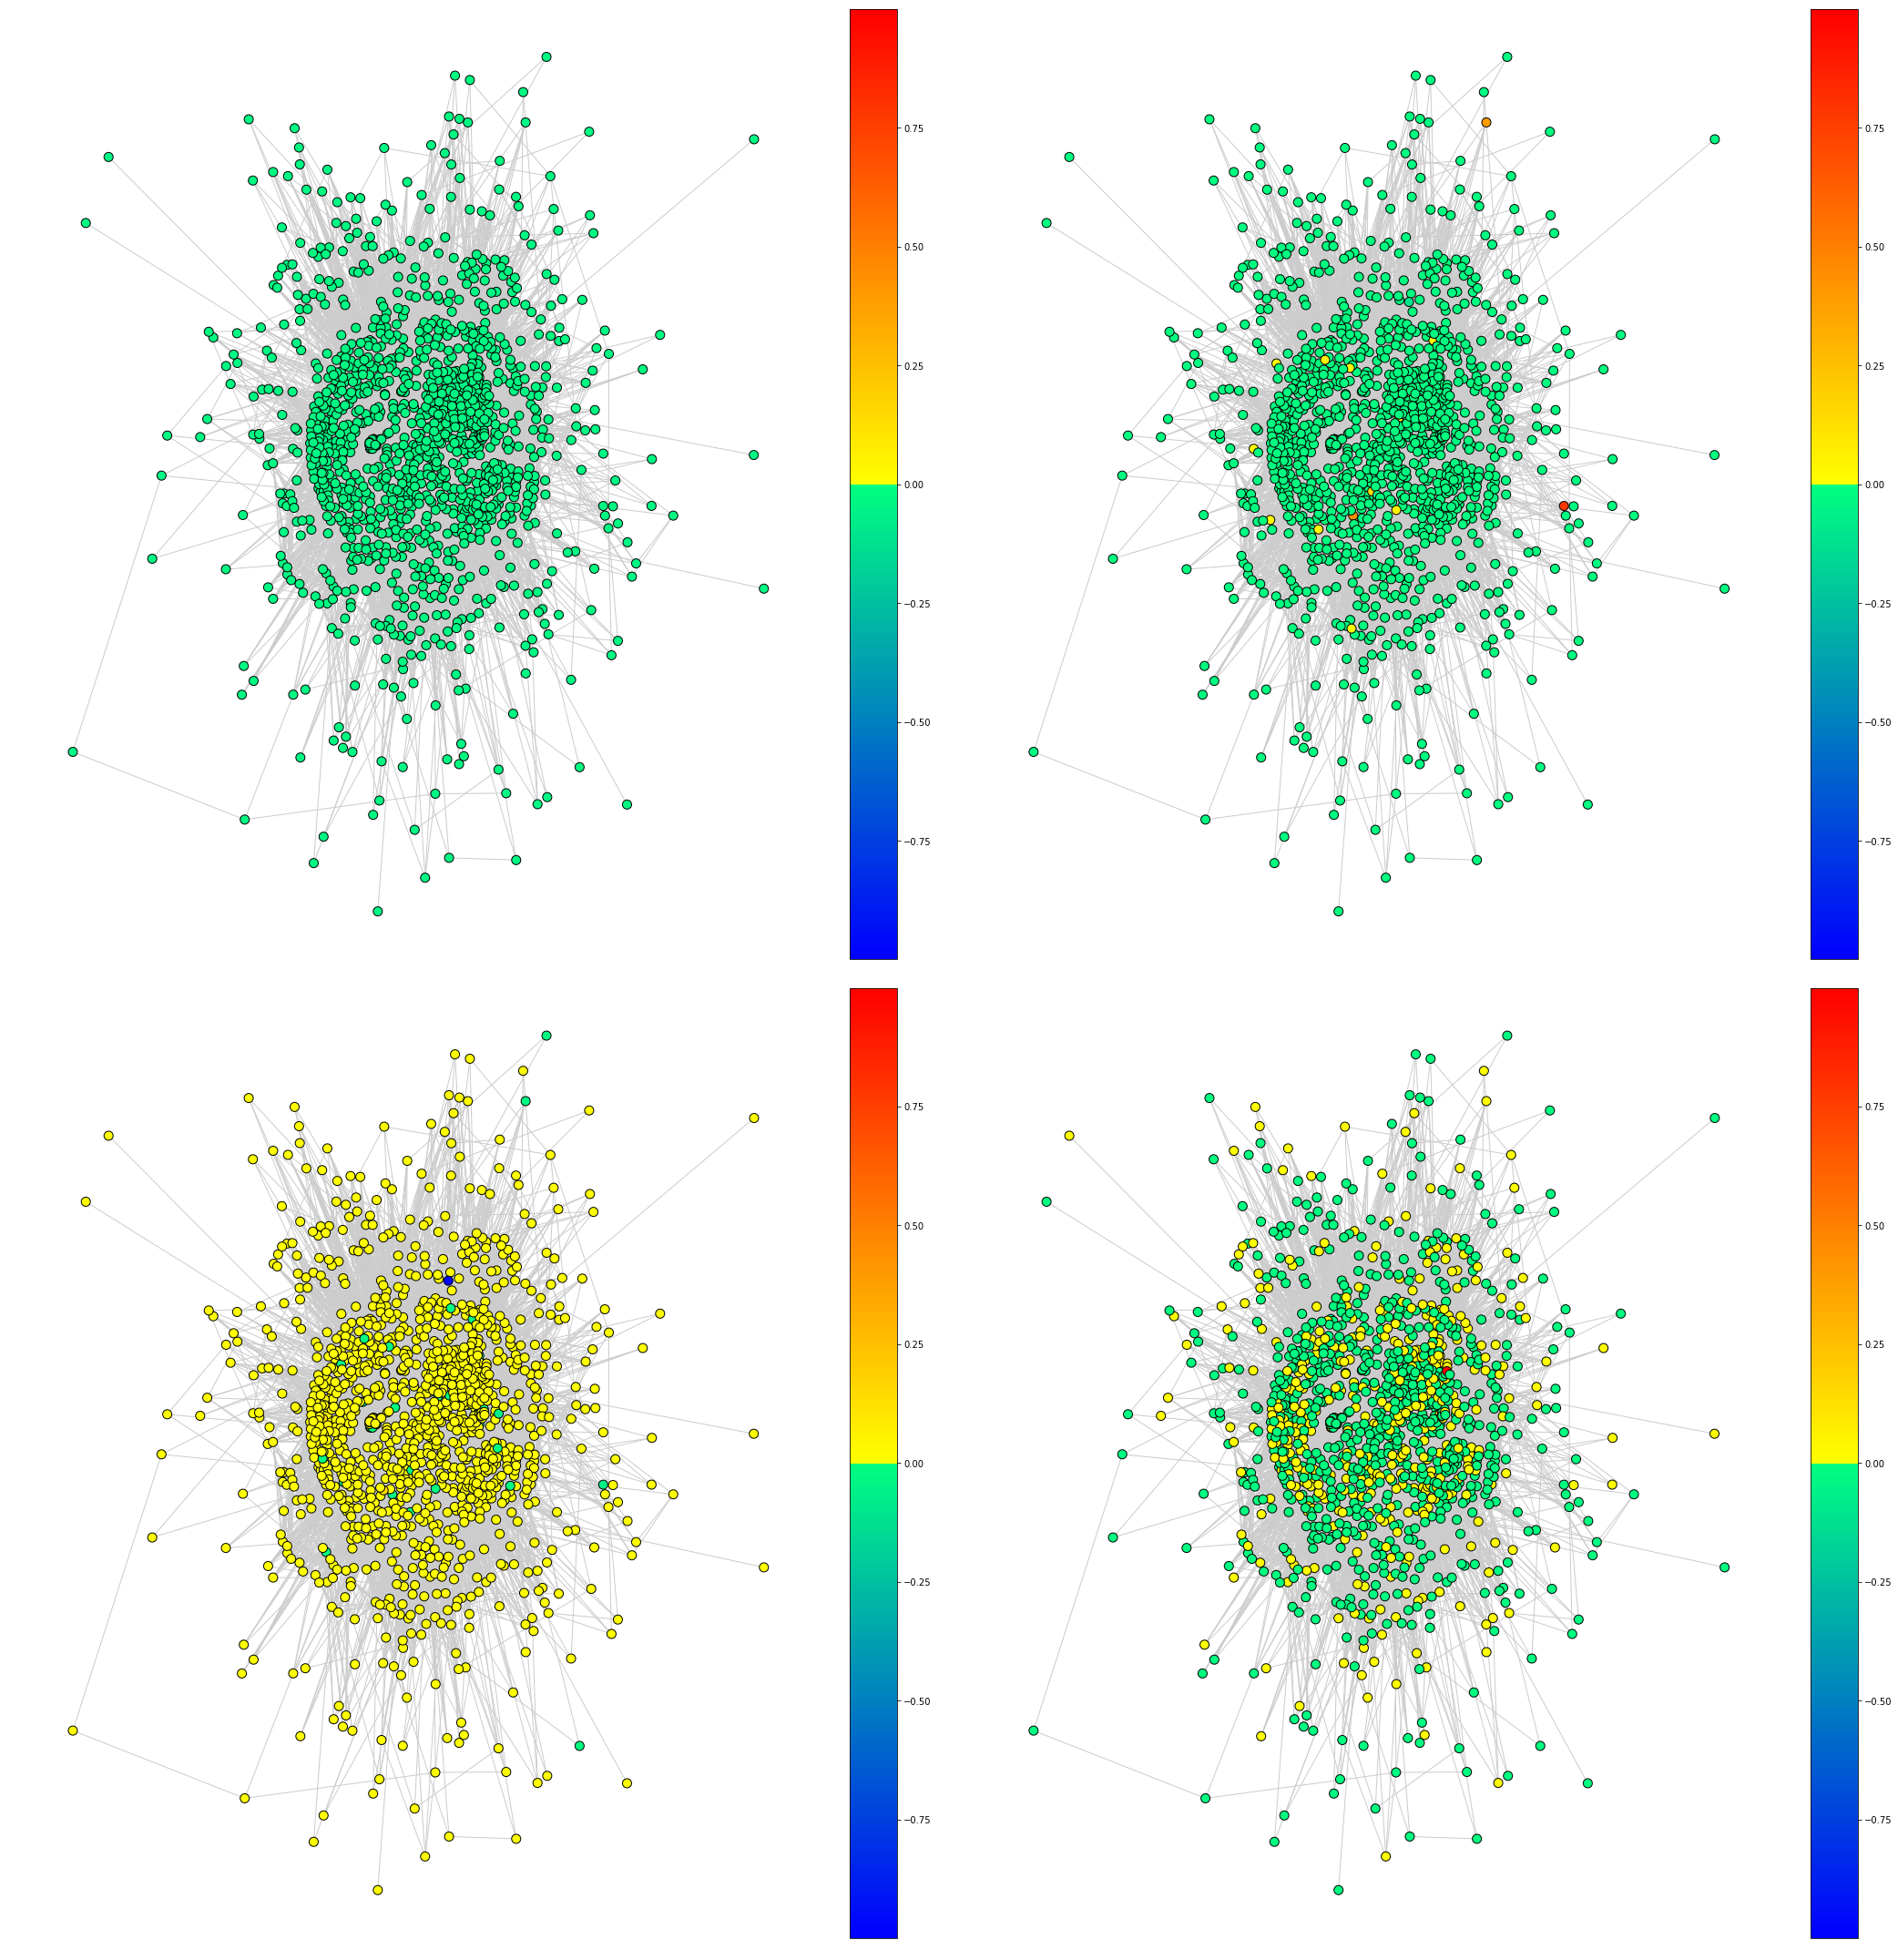
\includegraphics[scale=0.2]{images/iEC1344_C-4.png}
      \end{center}
      \caption{iEC1344 metabolic network}\label{fig:iEC1344_C-4}
\end{figure}

\begin{figure}[H]
      \graphicspath{ {images/} }
      \begin{center}
            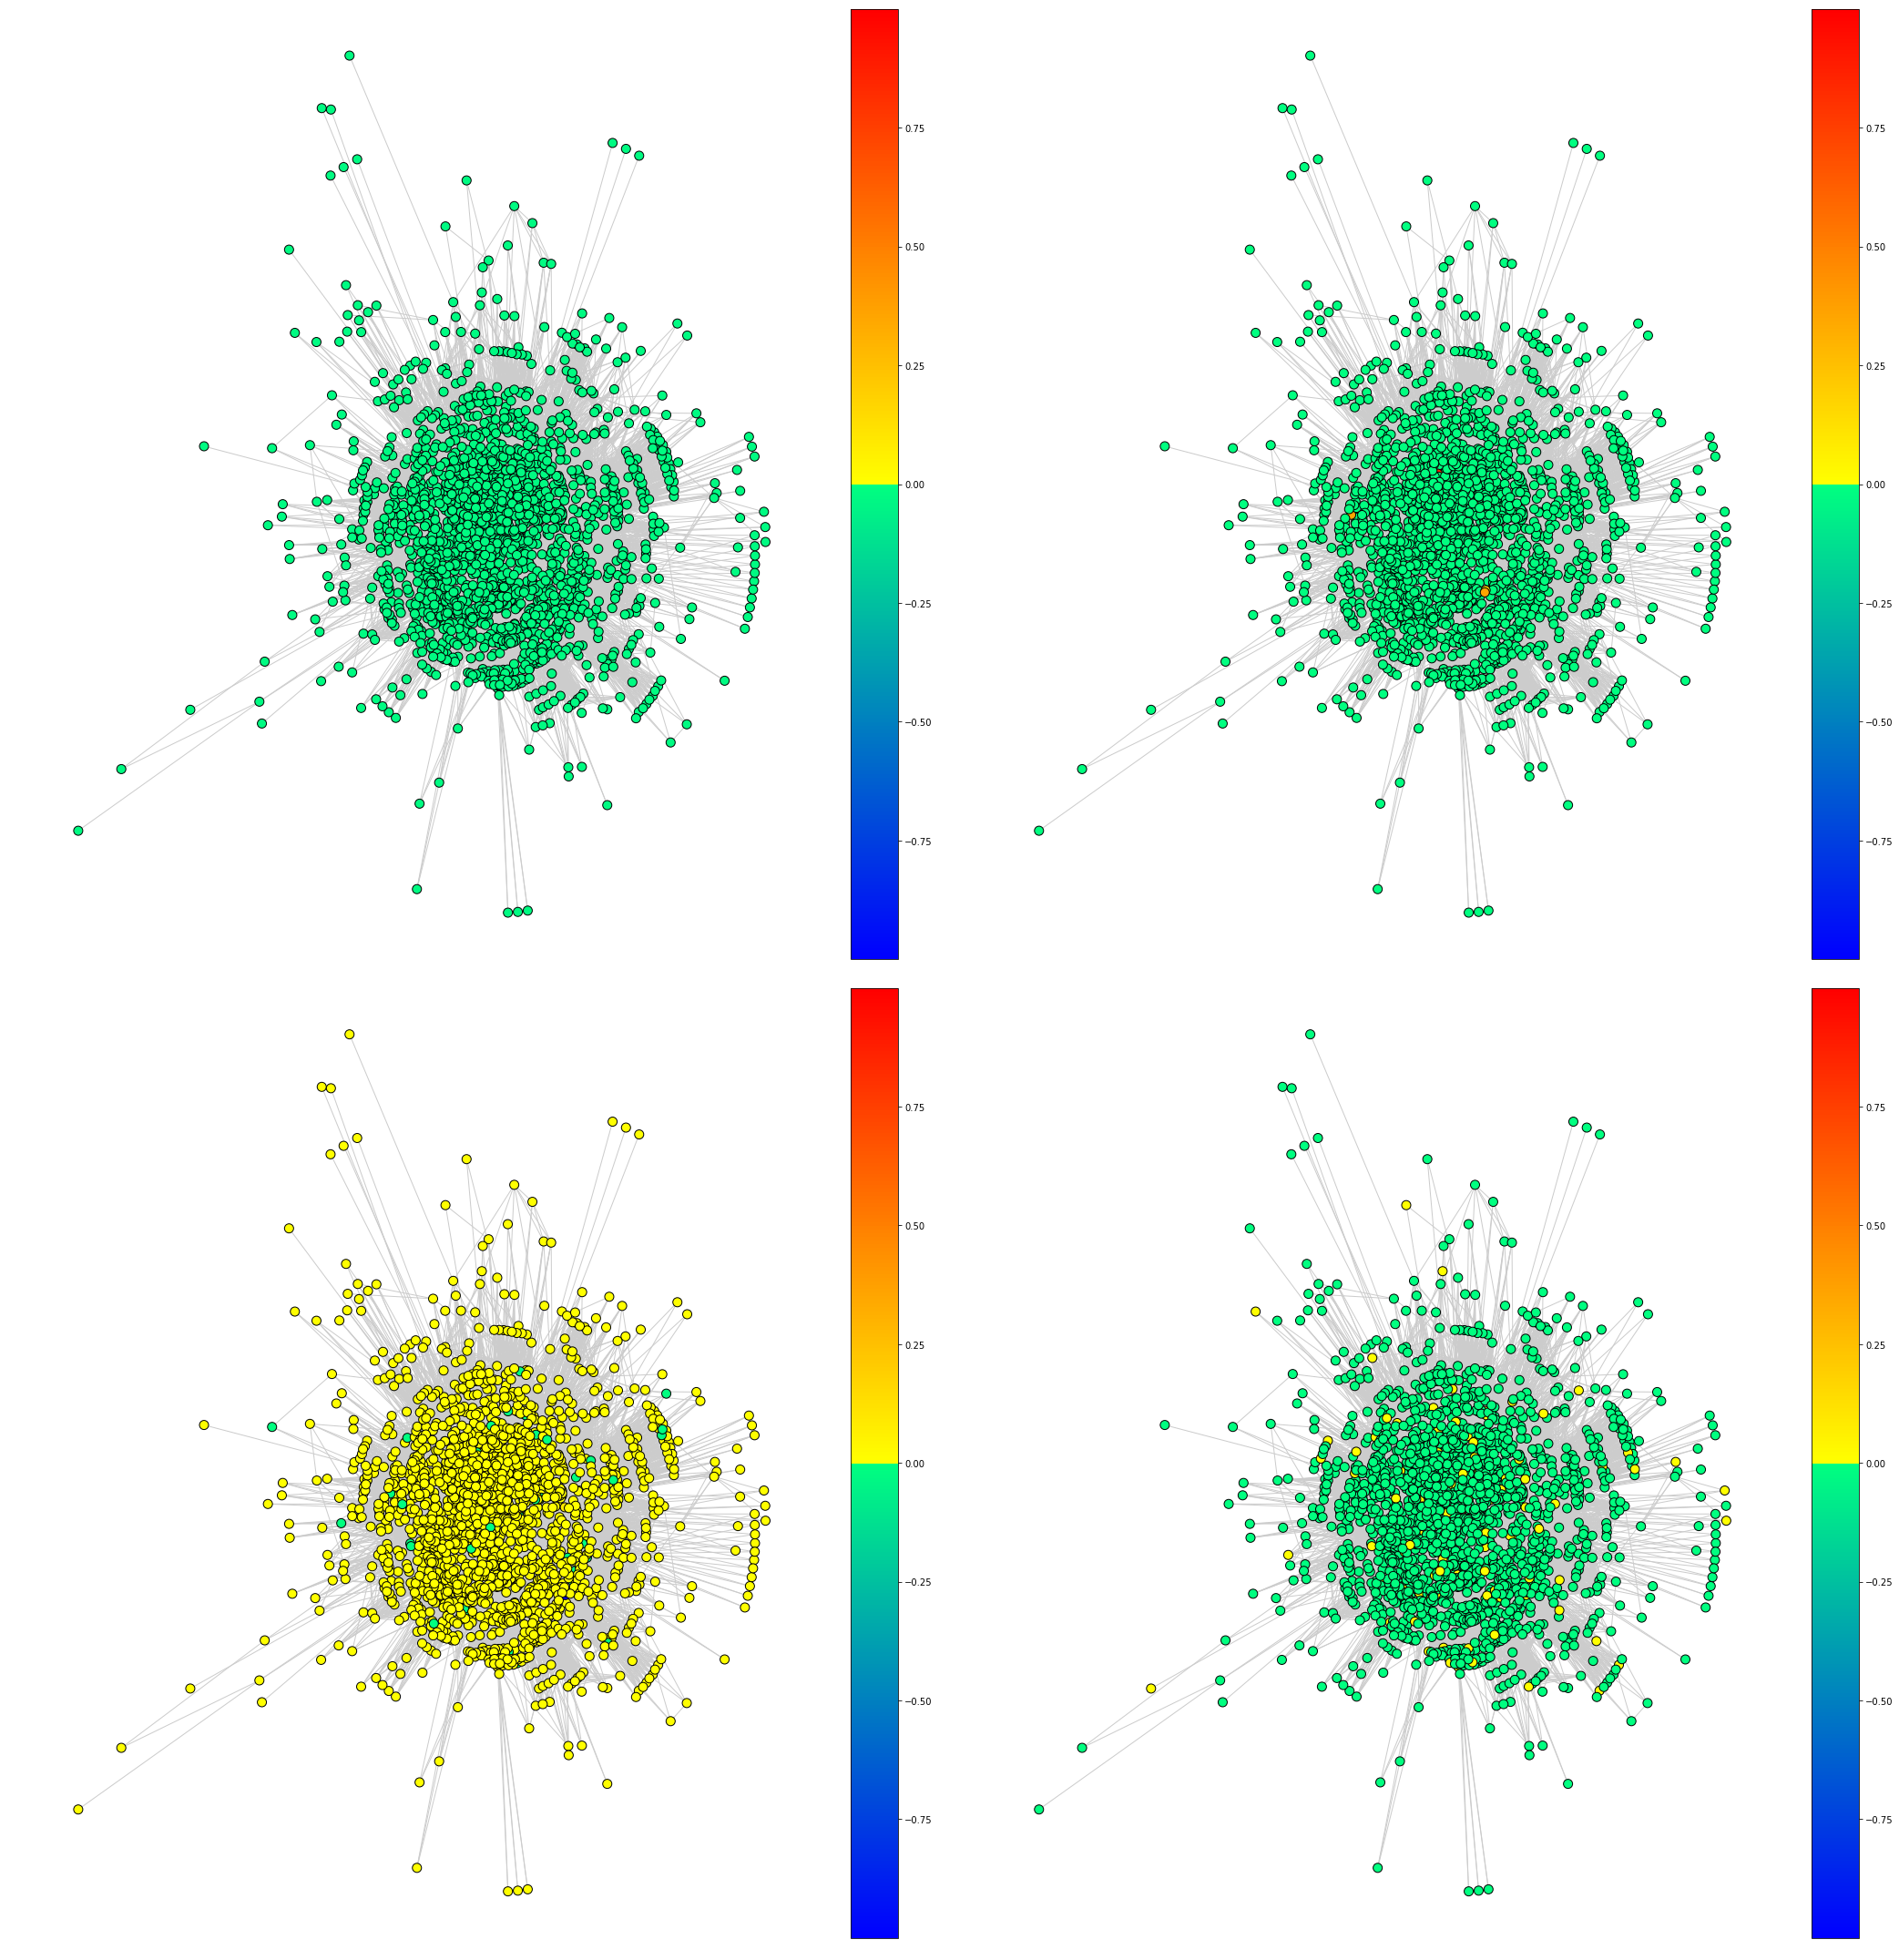
\includegraphics[scale=0.2]{images/Recon3D-4.png}
      \end{center}
      \caption{Recon3D metabolic network}\label{fig:Recon3D-4}
\end{figure}

\begin{figure}[H]
      \graphicspath{ {images/} }
      \begin{center}
            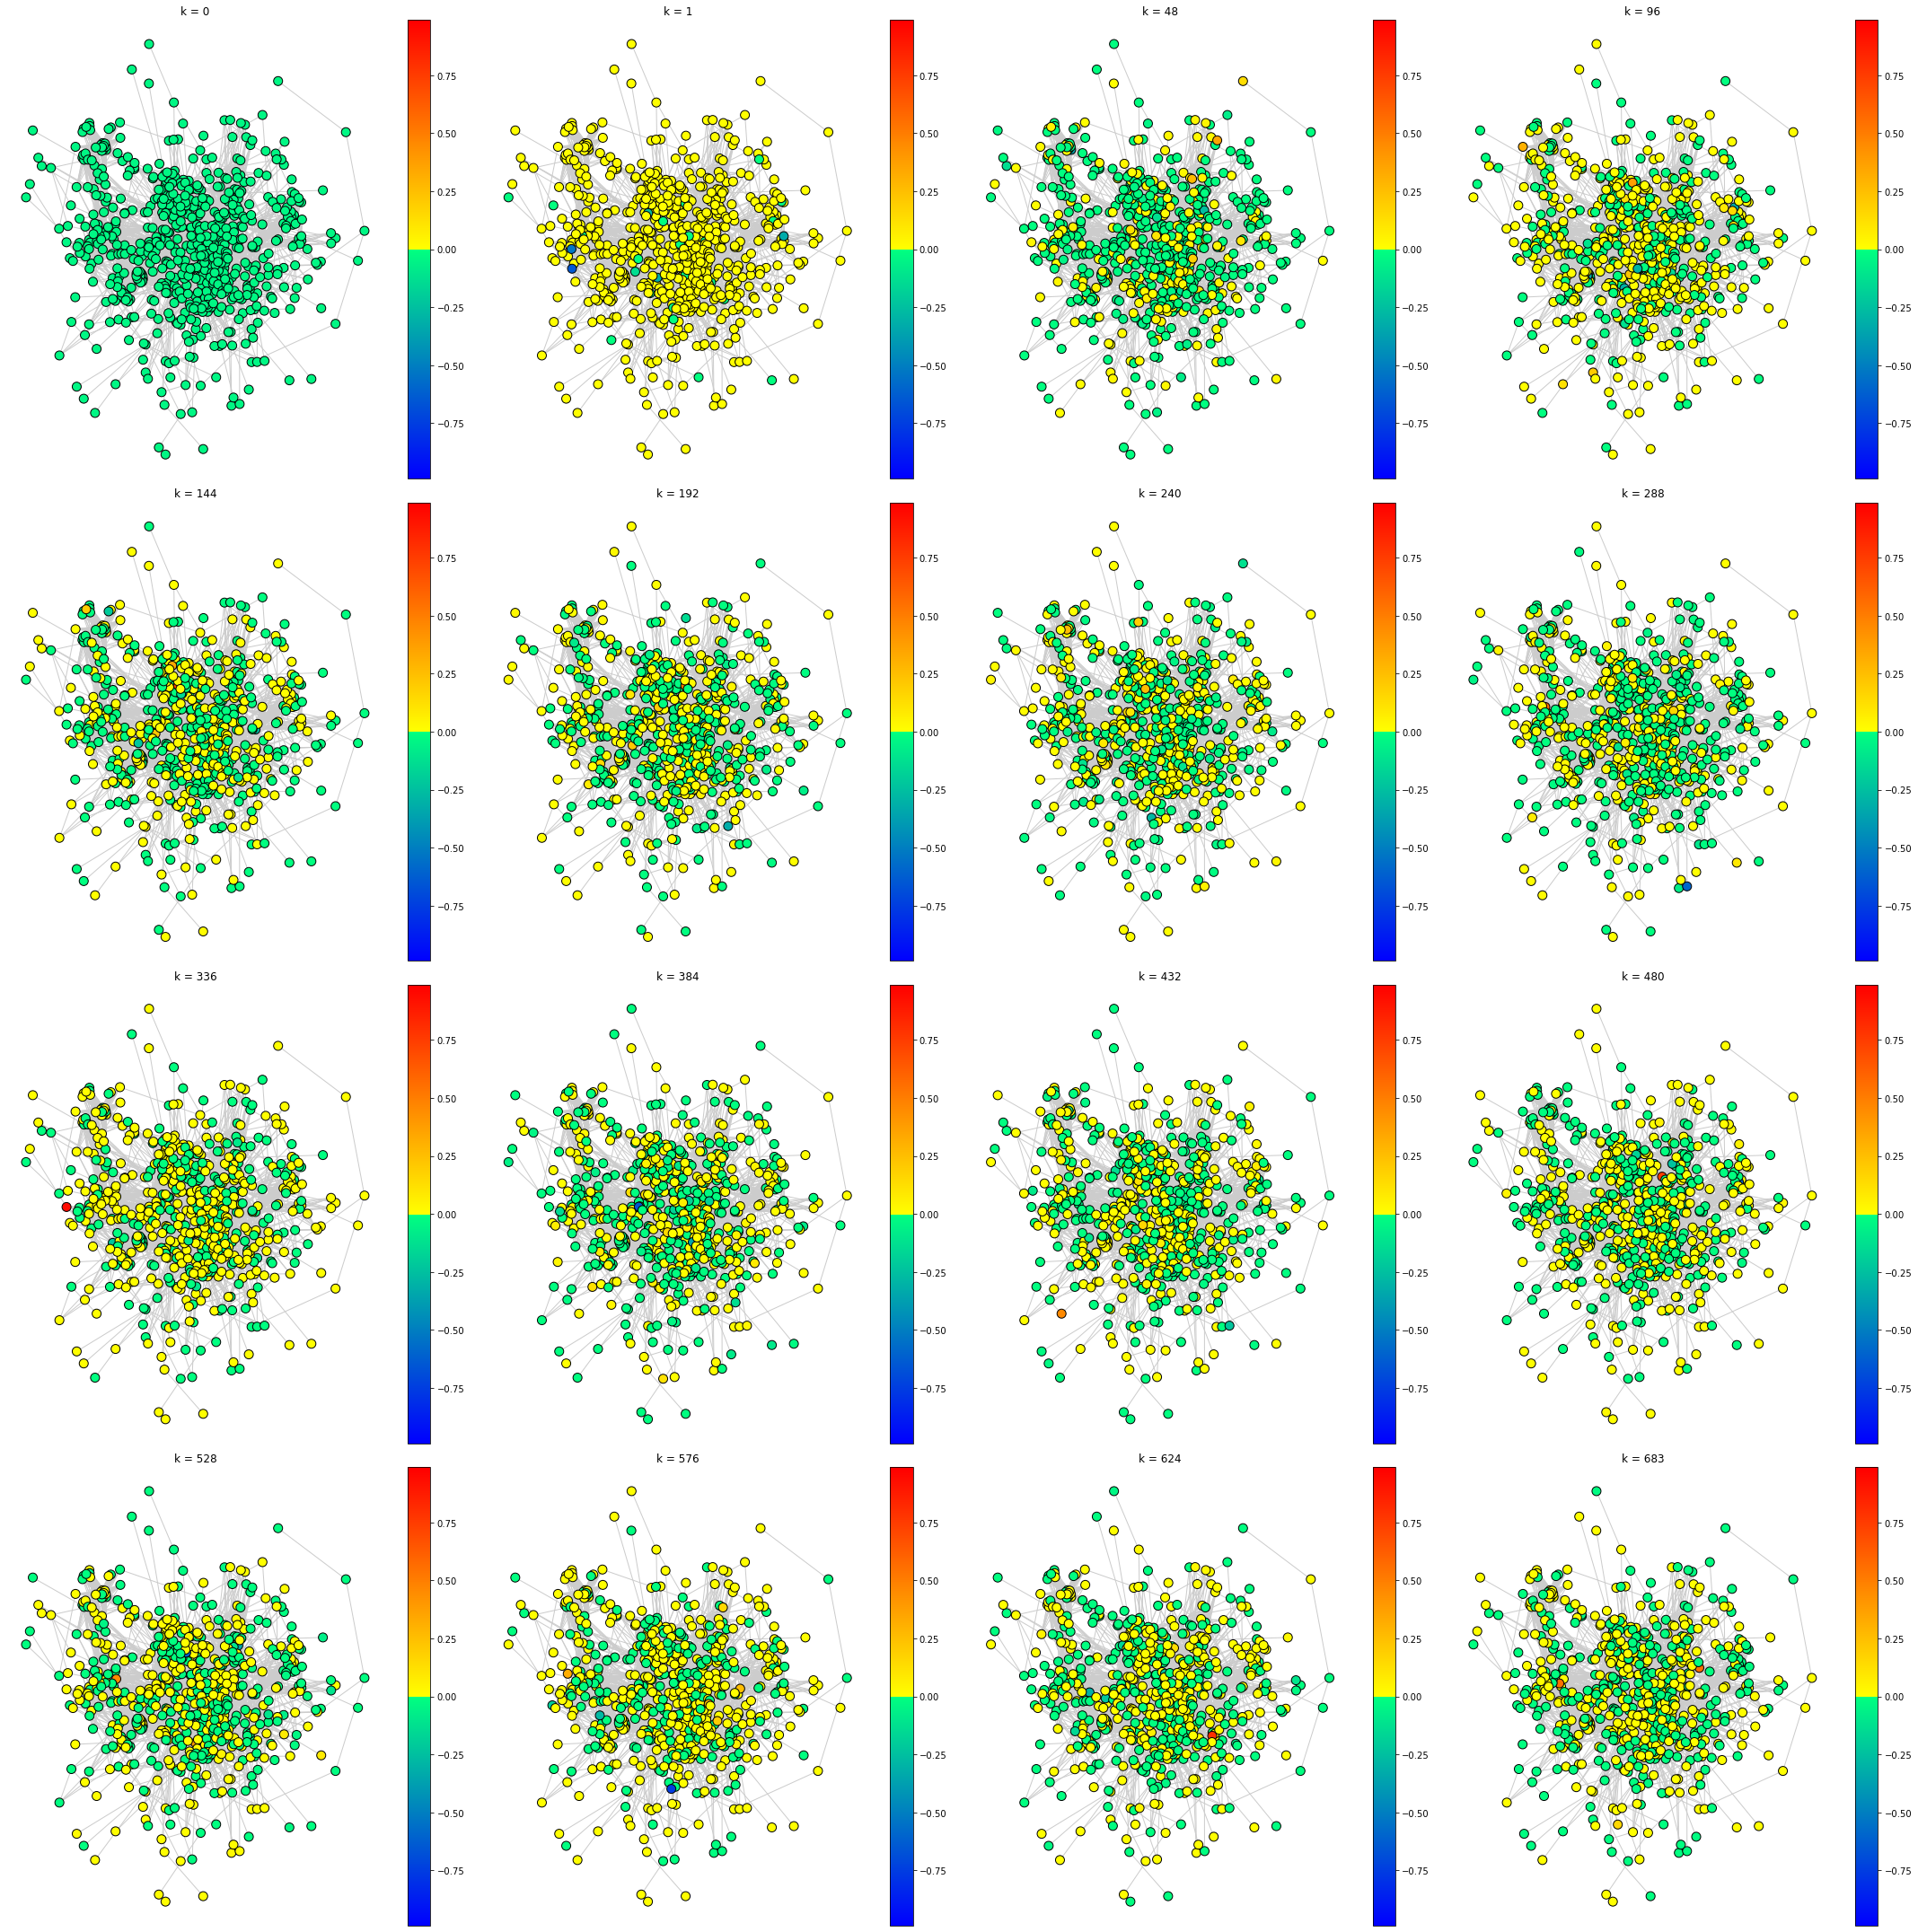
\includegraphics[scale=0.2]{iND750.png}
      \end{center}
      \caption{\textbf{Decreasing of the Smoothness.} Set a fixed step between graphs, the trend of smoothness decreasing is more obvious. The decreasing rate also seems to decline as index get larger.}
      \label{fig:iND750}
\end{figure}


\bibliographystyle{IEEEtran}
\bibliography{Library}

\end{document}
